\externaldocument {1chap}
\let\textcircled=\pgftextcircled
\chapter{User Study}
\label{chap:8}

\initial{T}o evaluate the difficulty of levels in the game it was decided to conduct the study with the users who should be able to solve the game of different levels. All levels of difficulty was assumed based on seen results of Savile Row Solver (implemented in Essence Prime).

The study involves multiple methods to make game harder in each level. In order to show that the conjecture is correct by using these methods it was needed to prove the following hypothesis:

H1: There are some parameters which can influence to the level of the hardness: size of the solution board, the amount of given information based on the percentage of the coloured cells on the board, and the last but not the least is the number of given clues on the top and left matrices. 

you can find this in example of chapter 1: \ref{ex:example1}\\
%----------------------------------------------------------------------------------------
%   Method: 
%----------------------------------------------------------------------------------------
\textbf{Method}\\
\textit{Participants:} \\
We recruited a sample of 12 participants from the School of Computer Science, University of St Andrews, where the number of males was 8 and females 4. 
Four of them had the experience on playing Nonograms before the study and the rest never played this game before.

\textit{Apparatus and Material}\\
The generated instances of Nonogram using various algorithms for producing different levels of the difficulty was displayed and printed on the papers to conduct the user performance study. 
Overall there were 5 levels: 

%----------------------------------------------------------------------------------------
%   EXAMPLE 1: Table
%----------------------------------------------------------------------------------------
\begin{table}
\centering
\begin{tabular}{ |c|c|c|c| }
     \hline
     Levels & Sizes (rxc)& Proportion coloured cells & Total number of clues\\ 
     \hline
     Level 1& 7x7 & 70 & 24 \\  
     Level 2& 7x7 & 70 & 31 \\
     Level 3& 7x7 & 50 & 20 \\
     Level 4& 7x7 & 50 & 36 \\
     Level 5& 7x7 & 70 & 48 \\
    \hline
\end{tabular}
\caption{Shows the properties of each level of Nonogram}
\label{table:nonogram_properties}
\end{table}


These 5 levels were generated to check the reliability of the assumed algorithms to generate different levels of difficulty of Nonogram measure by the time of solving them. In overall, we came out to three parameters which could be used to make the game more difficult:

\begin{enumerate}
    \item Having the same size the same number of coloured cells on the solution board, but having different number of clues per rows and columns, might make the game harder. 
    The program prompts the user to insert the size for the “solution board” and the percentage of the “coloured cells”, and can generate several instances. Some of them are with one solution and some of them with zero or many solutions. But we will consider only those which has only one solution.
    For the study with participants, in order to save the time for running through all possible combinations, it was decided to run through only 15 iterations and out of that range take two instances, which must have one solution, and one of them has the biggest amount of clues in top and left matrices and another is the smallest amount. The minimum amount of clues would be considered the easiest one and the maximum ones as the hardest from the list of generated instances with the same size and the same number of coloured cells. 
    This idea came because it was thought that if the amount of clues are less than it might mean that the values in the top matrix and left matrix are very big, which probably makes easier to find the intersecting parts of the big block and colour them at first steps of the solving process. (human logic). Otherwise the game is assumed to be harder, when digits in top and left matrix get smaller and it makes harder to colour the first steps of the game. 

    \item Another assumed parameter which might make the game more difficult or easier is the percentage of coloured cells. If the amount of black cells on the solution board are small, then the generated instance will have less amount of information to solve the game, this makes the game harder to solve, and oppositely if the amount of the coloured cells are big, it makes the instance more full of information and easier to solve the game.

    \item The last idea about the way to make game more difficult is the the size of the Nonogram. If the size of the game to increase and to keep the same proportion of the coloured cells as for previous levels. It will demonstrate whether the instance takes more time to solve it.
\end{enumerate}

In order to check whether these parameters are affecting to the level of difficulty and in which direction. Each of the five levels were thought in the way so that we could check only one parameter at a time. 
\begin{itemize}
    \item \textbf{Level 1} and \textbf{Level 2}, as it was mentioned before, they all has only one solution, which means they are solvable. The same size and the same proportion of the coloured cells (number of rows: 7, number of columns:  7, 70\% of the solution board should be coloured), but they have different amount of clues. That will allow us to compare the influence of the amount of clues to the level of difficulty. Level 1 has the minimum amount of clues out of 15 instances (24 clues, including all clues from top and left matrices). Level 2 the largest amount of clues out of those 15 instances (31 clues)(see Table \ref{table:nonogram_properties}).
    \item \textbf{Level 3} and \textbf{Level 4}  have one solutions, the same size (rows = 7, columns = 7) as Level 1 and Level 2, but they have less information given at the beginning. Since only 50\% of the solution board will be coloured. Level 3 has the minimum amount of clues and Level 4 has the maximum
    Later for analysis we could compare Level 1 with Level 2 and Level 3 with Level 4 to compare the time spent to solve them with different number of clues. 
    Since Level 1 with Level 3 and Level 2 with Level 4 have the same size and the minimum amount of clues, it is more likely to compare their times to check the influence of given percentage of coloured cells to the levels of difficulty as well. 
    \item \textbf{Level 5} was generated to check how size of the board can change the level of difficulty. For this level it was taken the instance out of 15 with one solution and smallest number of clues, where the size is 10x10 and the proportion of coloured cells is 70\%. This level can be compared with the level 1, which also has the smallest amount of clues out of its instances and 70\% of coloured cells, but the size is smaller (i.e. 7x7). 
\end{itemize}

\textit{Procedure:} \\
At the beginning of the experiment the participant was explained with the rules of the game. 
All participants were given with identical instances and in the same order, assuming that they are allocated in the reasonable order with the respect to the levels of difficulty. In overall participant had to solve five instances and record the time spent to solve the puzzle. For each instance the participant was given with maximum 5 minutes to solve it. In total for the entire experiment each person should spend 25-30 minutes (including the explanation of the rules). To prevent the cases of spending too much time on solving one instance it was decided that the user will spend at maximum 5 minutes per instance, and in total should not spend more than 30 minutes for the experiment including the explanation of rules and fast survey. Five minutes per instance was chosen, since in general an experienced user who knows the rules and can solve the instance completely can spend 2-4 minutes. In general the participant could have three possible outcomes of solving the instance:

\begin{enumerate}[(i)]
    \item successfully solved instance in less than 5 minutes;
    \item not completed instance due to time limitation (spent 5 minutes exactly); 
    \item not completed due to found mistake, which is normally hard to fix (generally was happening in less than 5 minutes.)
\end{enumerate}

In the cases when the participant solves the game in less than 5 minutes, he can record the obtained time and with restarting the timer starts the next instance. In the case of the second outcome the user just must stop the game and move to the new instance. In the third case the user just marks that he/she couldn’t solve it and moves to the next level. 
Even if users will not complete the puzzle this will still allow us to know how difficult the game was since we still can see how correctly and how much of the board was solved in this maximum 5 minutes time range. 

At the end of the game the participants were asked several questions how they would rate the instances in terms of their levels of hardness and whether they played this game before. 

\textbf{Results}
In total we collected around of \textbf{4 hours 13 minutes} data (25 minutes maximum per participant, the number of which was 12). Just some of the users completed the experiment faster. 

After the experiment was conducted all the data was gathered to the Excel spreadsheet, where we written the index of the participant and the amount of time spent per each level. Since some of the levels were not completed and some of the levels failed for some users and the maximum limit per instance was 5 minutes. Thus the user could not exceed the limit 5 minutes, it was decided to denote those who just didn’t complete it fully with 6 minutes and those who failed were denoted with 7 minutes. Since it shows that the level became so difficult enough so that the participant would need more time to complete it or even probably more time to fix the mistake. Therefore the table does not have any “Not Available” data. This approach was decided just for the sake of easiness. Thus all “Not Completed” and “Failed” states would be denoted also with longer time, 6 and 7 minutes respectively.

Therefore, in the filtered process we are still able to check when the time is equal either to 6 or 7 put them on different list from the other time less than 6 minutes, i.e. successfully completed lists.

Since we have got the information about previous experience in this game, we can separate people who played this puzzle game before from those who saw this game first time during the experiment. Despite the experience the user still should spend longer time on the more difficult levels. However, since we asked participants to stop the game despite they did not complete the level once the 5 minutes reached, we cannot rely on it since for some participants all levels were taking longer than 5 minutes, due to their lack of experience in this game. Moreover the people who had experience in this game has more consistent results, while the people with no experience might be improving in each level, which might skew the assumption of making game harder.

Therefore it is probably better approach to split the participants to two groups and analyse the people with more experience separately from all. And then for general analysis, it is still possible to consider all data together. 

Initially it was split to two groups and checks how well the participants solves the game.

\begin{table}
\centering
\begin{tabular}{ |c|c|c|c| }
     \hline
     Level & Experienced& Not Experienced & Total\\ 
     \hline
    1
    & 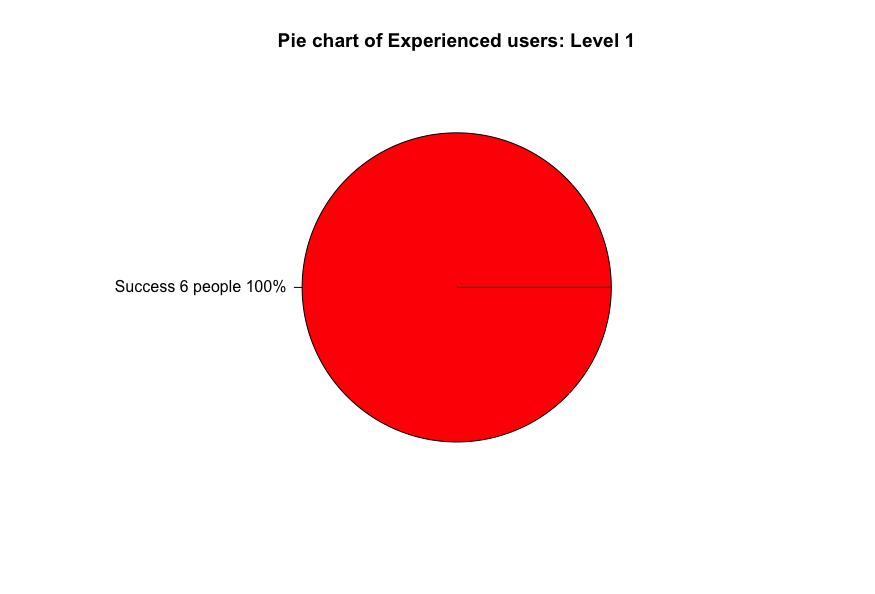
\includegraphics[width= 0.3\textwidth]{img/L1_exp.png}
    & 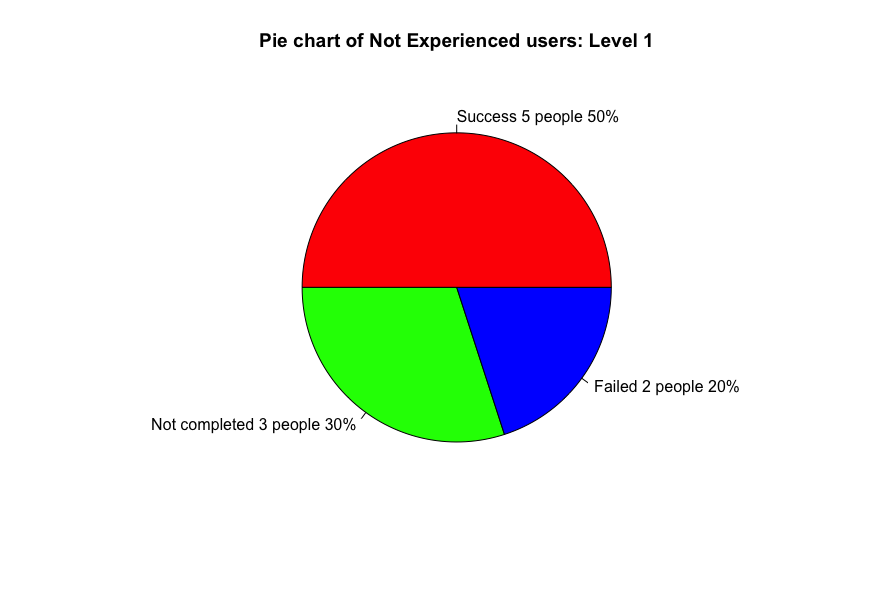
\includegraphics[width= 0.3\textwidth]{img/L1_NE.png} 
    & 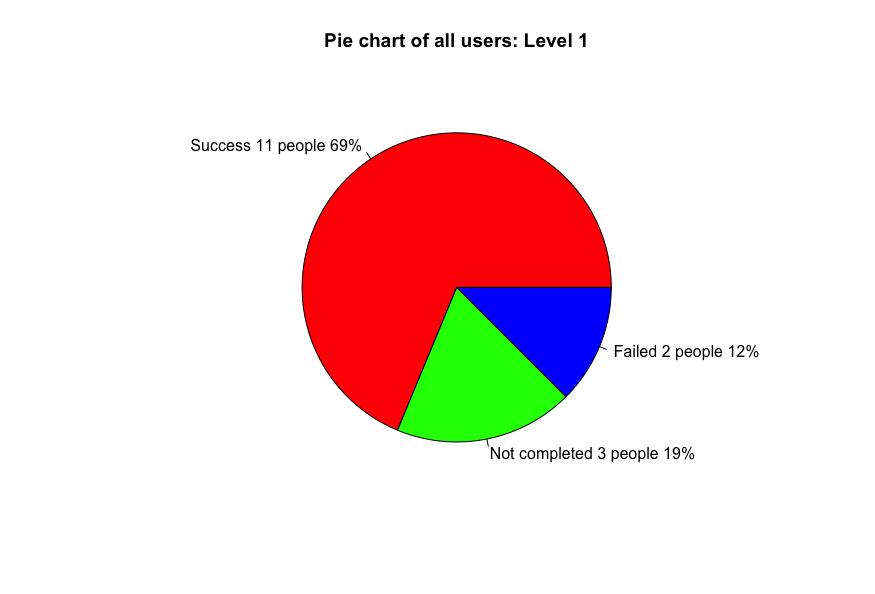
\includegraphics[width= 0.3\textwidth]{img/L1_all.png}\\  
    2
    & 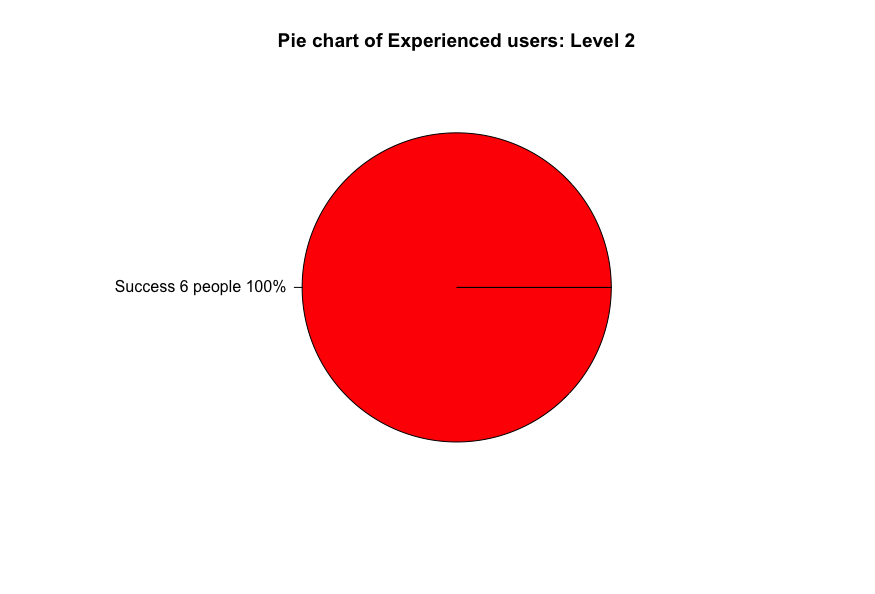
\includegraphics[width= 0.3\textwidth]{img/L2_exp.png}
    & 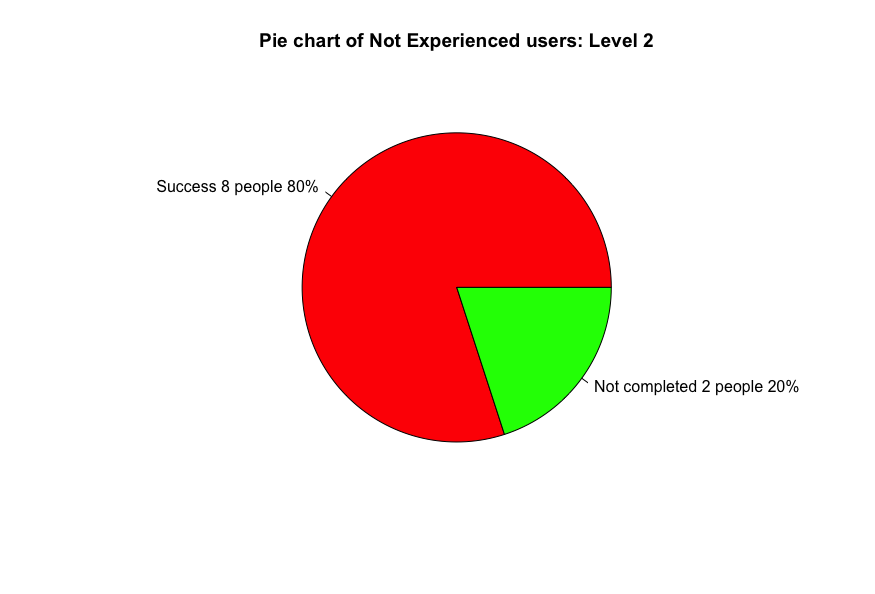
\includegraphics[width= 0.3\textwidth]{img/L2_NE.png} 
    & 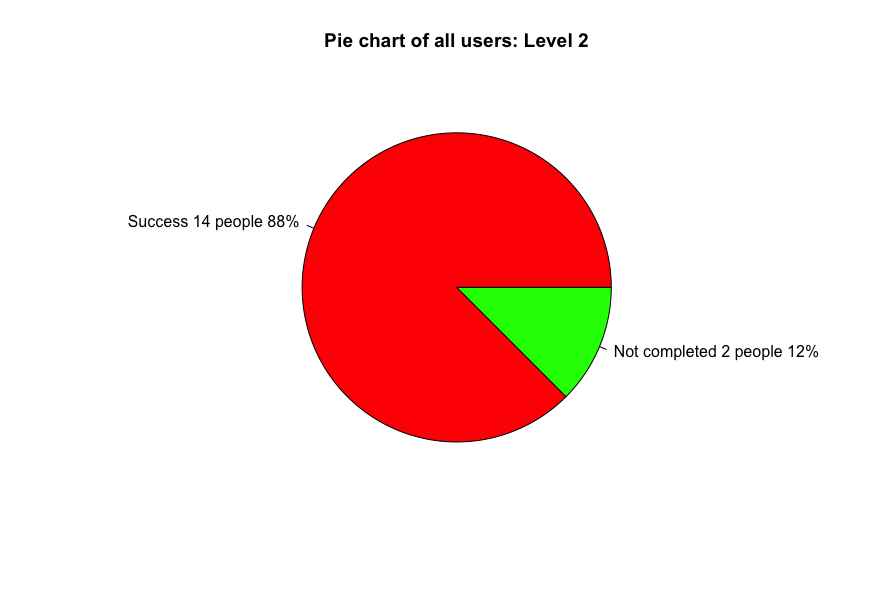
\includegraphics[width= 0.3\textwidth]{img/L2_all.png}\\  
    3
    & 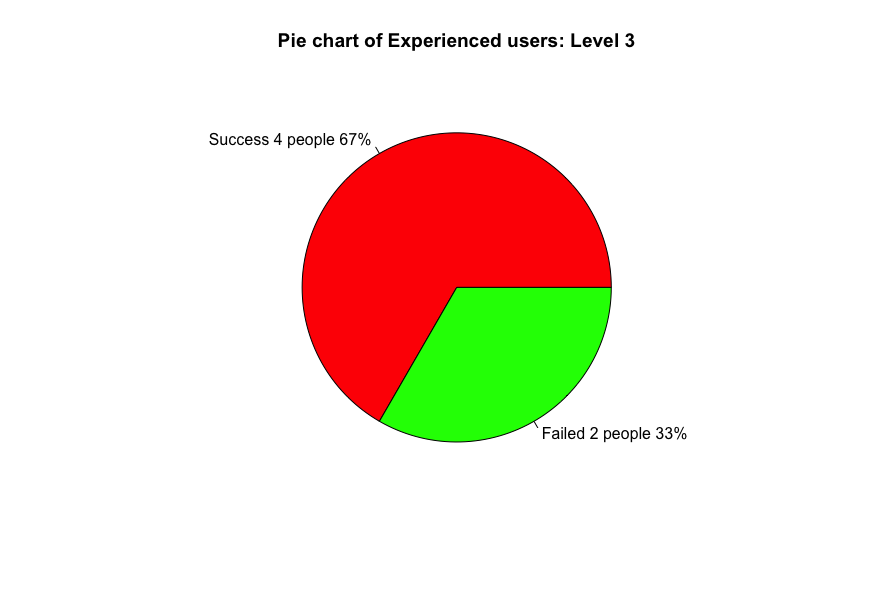
\includegraphics[width= 0.3\textwidth]{img/L3_exp.png}
    & 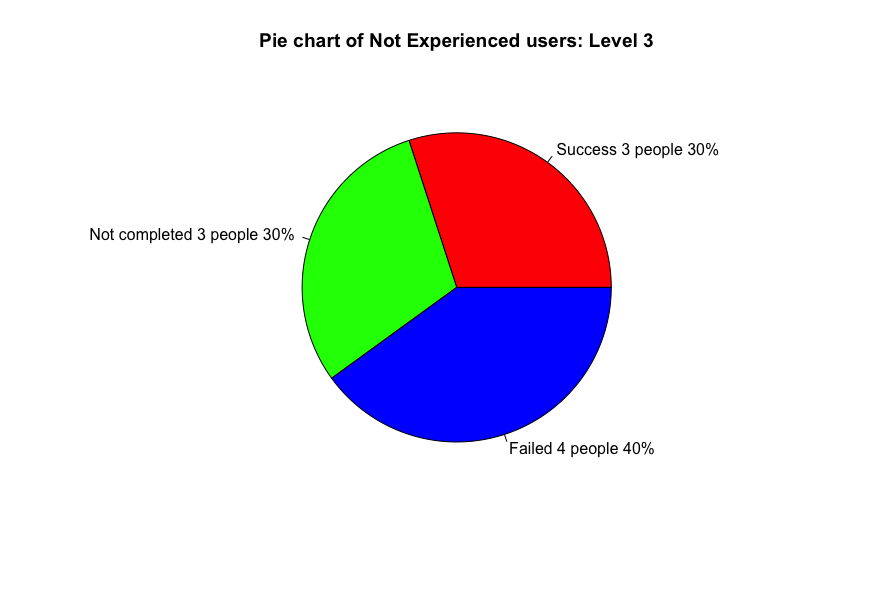
\includegraphics[width= 0.3\textwidth]{img/L3_NE.png}
    & 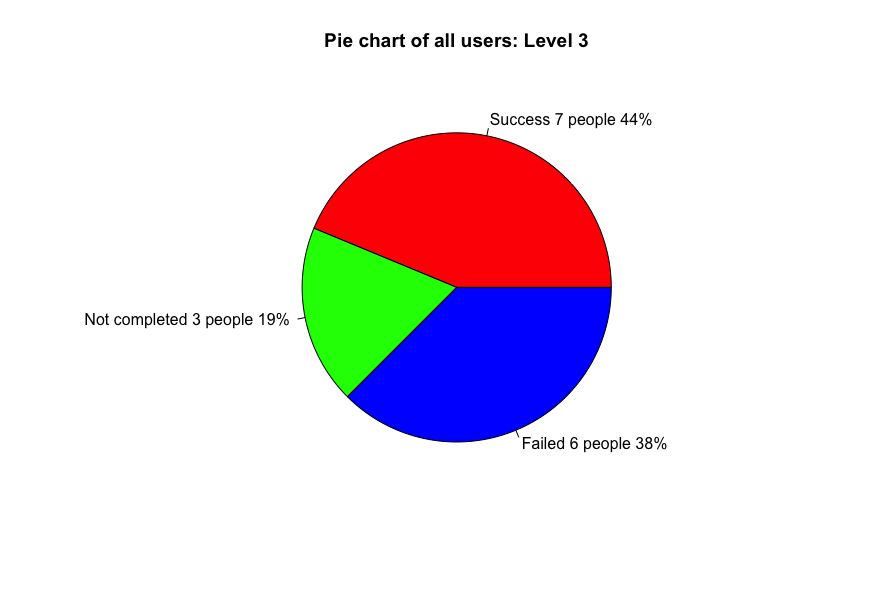
\includegraphics[width= 0.3\textwidth]{img/L3_all.png}\\  
    4
    & 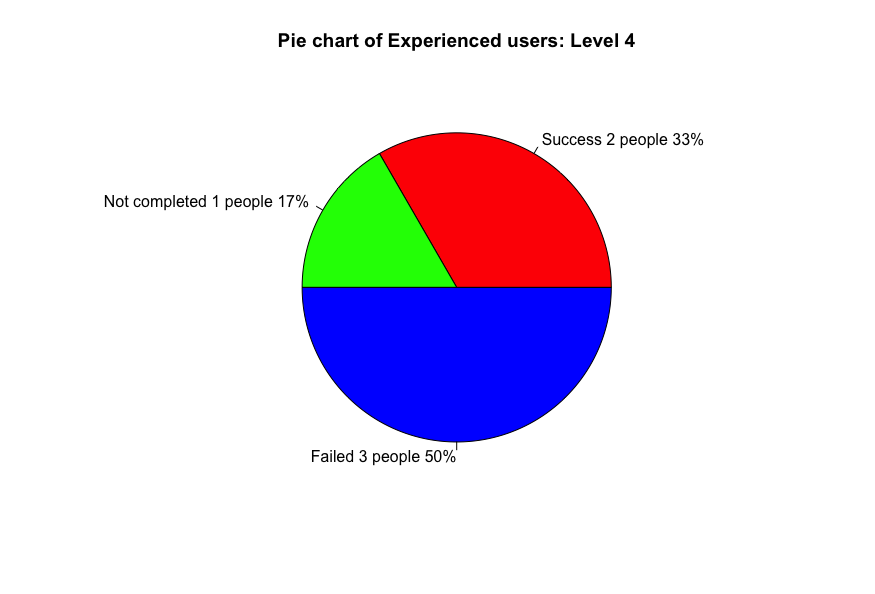
\includegraphics[width= 0.3\textwidth]{img/L4_exp.png}
    & 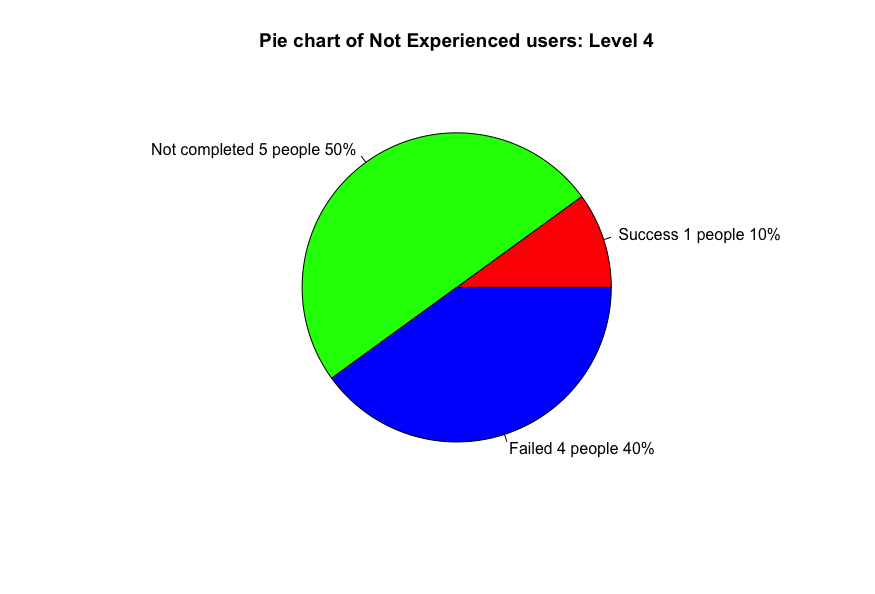
\includegraphics[width= 0.3\textwidth]{img/L4_NE.png}
    & 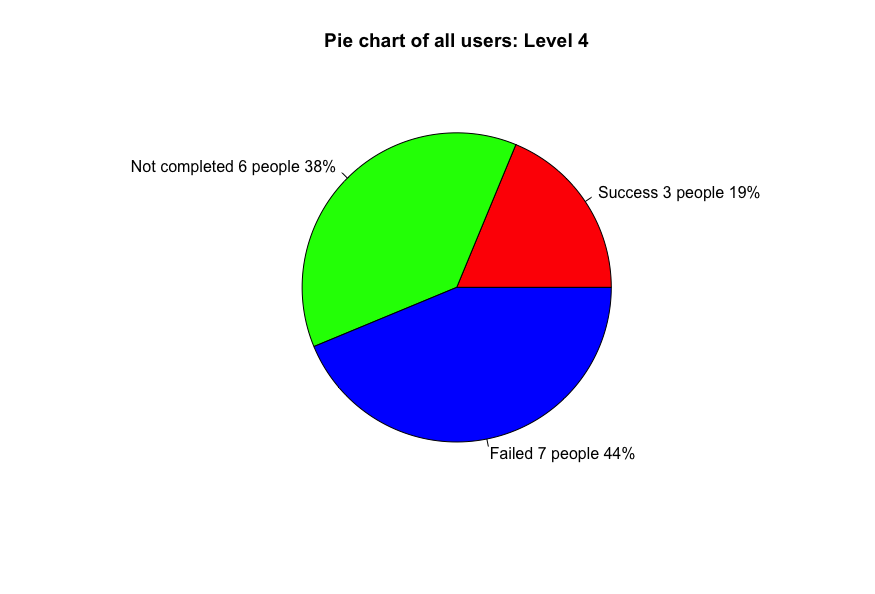
\includegraphics[width= 0.3\textwidth]{img/L4_all.png}\\
    5
    & 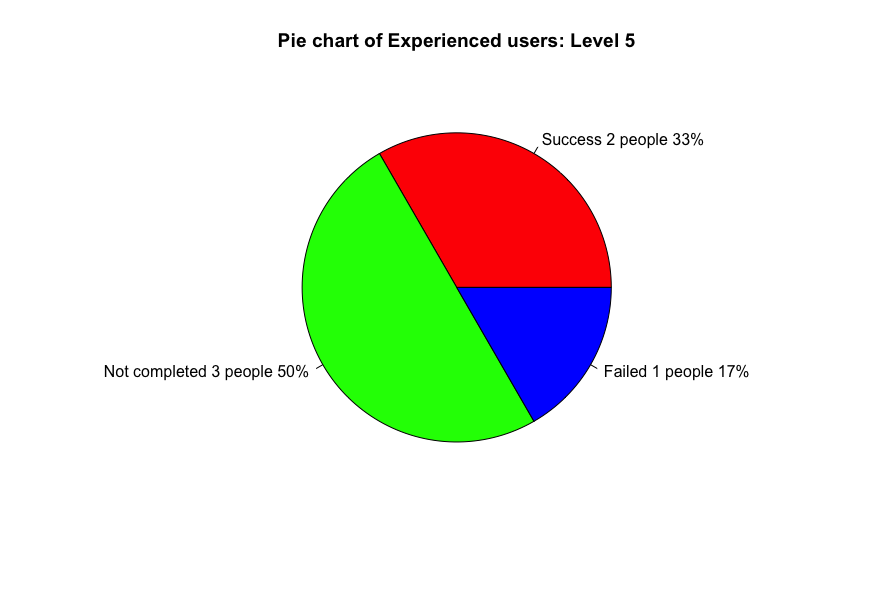
\includegraphics[width= 0.3\textwidth]{img/L5_exp.png}
    & 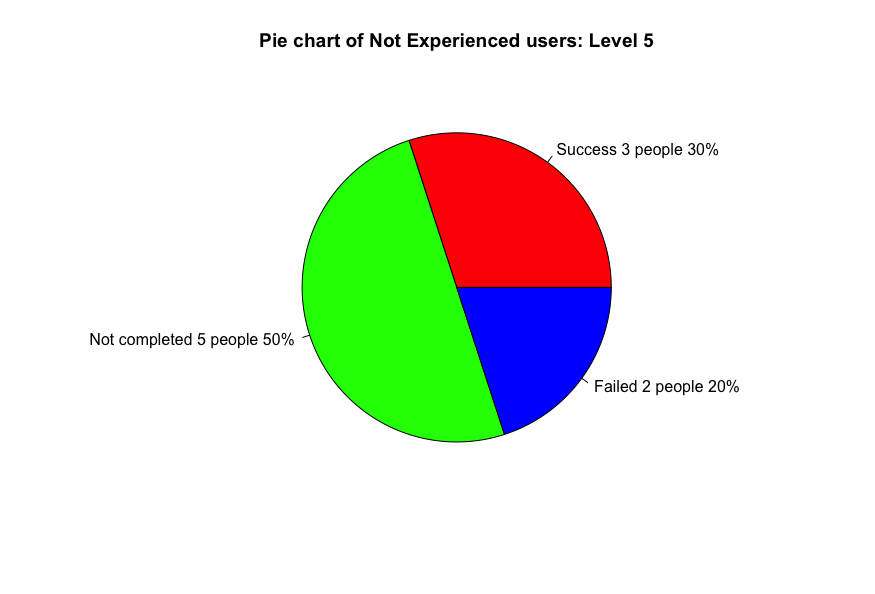
\includegraphics[width= 0.3\textwidth]{img/L5_NE.png}
    & 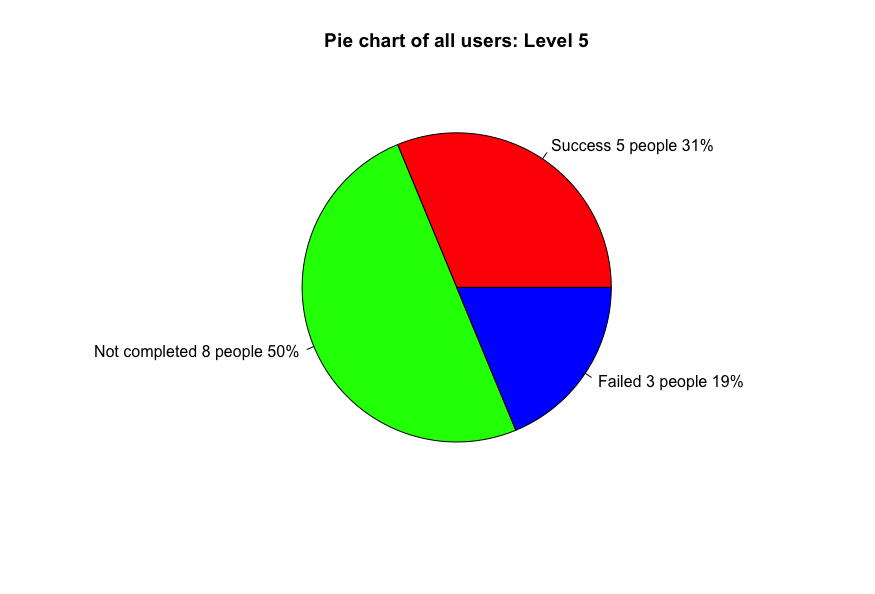
\includegraphics[width= 0.3\textwidth]{img/L5_all.png}\\  
    \hline
\end{tabular}
\caption{The performance of each level for experienced, not experienced and all together}
\label{table:piecharts_all_levels}
\end{table}

Accordingly all these pie charts in each level the proportion of successfully completed people in the list of experienced people is more than in the list of not experienced people. 

Level 1 and Level 2 are the most easiest, since they have the smallest given size and the biggest percentage of coloured cells, which assumed to make game easier. Accordingly the list of experienced people, in both levels all users completed the game successfully. However, in the list of the non experienced people , it can be seen that the number of successfully completed the game in the Level 1 is less than in Level 2, which could be explained due to their learning skills.

Level 3 and 4 definitely gets harder in comparison with levels 1 and 2, since even in the list of the experienced people the amount of successfully completed is reduced. In the Level 3 it is 75\% completed and 25\% just did not complete it due to time limitation, while in the Level 4 the percentage of successfully solved game people reduced sharply to 25\% only, 25\% did not complete and 50\% failed. This demonstrates our belief that the incrementation of amount clues makes the game a bit more challenging. However, for some reason the amount of failed in level 3 is 50\% and in Level 4 is 38\%, which probably tells that Level 3 is not easier than Level 4. Therefore, these pie charts does not clearly demonstrate that the theory of more clues makes the instance more difficult to solve. 

In case if it possible to compare Level 1 with Level 3 or Level 2 with Level 4, then it clearly could be stated that the number the reduction of the coloured cells proportion makes game harder. Since the number of successfully completed people decreases in both columns, experienced and not experienced participants.

Level 5 for experienced people was the same, it was one person who still solved it in less than 5 minutes, but it shows that level 5 is easier than Level 3 and Level 4 since there is no people who could fail it. The rest just did not complete it. While in the Level 4, 50\% of the experienced people just failed it. For non experienced people the percentage of successfully completed level 5 is more than in level 4 and the same as in level 3. However the number of failed people is much less than in level 3 and 4. 

Also better to check the correlation between the levels of difficulty and three suggested parameters. For that it was decided to use simple T-test and visualise them on the boxplots, which will make them easier to analyse.

\begin{figure}[h]
\centering
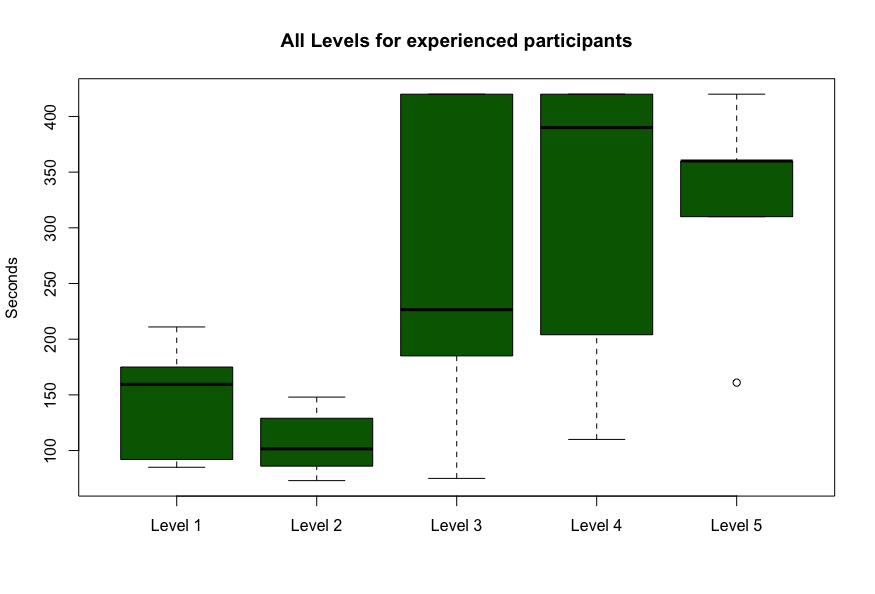
\includegraphics[width= 1.0\textwidth]{img/boxplot_all_experienced.png}
\caption{Boxplot for entire data of all levels}
\label{fig:boxplot_wholedata}
\end{figure}

The boxplot demonstrates the time spent for each level of experienced participants. People spent more time in Level 1 rather than in Level 2, which probably means that the idea of adding clues is not really demonstrates the ability of making the game more difficult. 
Definitely the means of Level 3 and Level 4 are higher and there is more possibilities that some people even failed it or did not complete. Thus the idea of giving less information by setting less percentage of cells on the instances is more likely will make game more difficult. The last Level 5 has less mean value than for Level 4, which also makes sense since the Level 5 just should take more time so solve than Levels 1 and 2, but still be easy solvable. 

The graph 1 is more reliable, since it matches the opinions of the participants who say that Level 2 was easier than Level 1, and Level 3 is easier than Level 4. Thus it is quite confusing to proof that the more number of clues will make the game harder. Level 5 is easy in general as Levels 1 and 2 but just will take more time because of bigger size. 
Therefore the most of the people would change the order of the game to placing in this order (see Table 3). This order seems to be reasonable, since in Level 5 there is less people who failed the game. The most of them were failing in levels 3 and 4 since they are much harder and accordingly the survey people feel in level 3 and 4 that they most of the time guess randomly at some steps and traverse back to get right answer, and because of that they are failing.\\



%%%%%%%%%%%%%%%%%%%%%%%%%%%%%%%%%%%%%%%%
% -- previous--
% \begin{center}
% \begin{table}
% \begin{tabular}{ccc}%
% \begin{tabular}[t]{|c|c|c|}
% \hline
% $\textbf{Levels}$&$ \textbf{Means}$&$\textbf{Time}$\\
%                  &$ seconds $            &$MM:SS$\\
% \hline
% $Level 1$ & $237.9$ & $3:57.9$\\
% $Level 2$ & $169.8$ & $2:49.8$\\
% $Level 3$ & $324.6$ & $5:24.6$\\
% $Level 4$ & $353.9$ & $5:53.9$\\
% $Level 5$ & $337.8$ & $5:37.8$\\
% \hline
% \end{tabular} 
% &
% \begin{tabular}[t]{|c|c|c|}
% \hline
% $\textbf{Levels}$&$ \textbf{Means}$&$\textbf{Time}$\\
%                  &$ seconds $            &$MM:SS$\\
% \hline
% Level 1 & 237.9 & 3:57.9\\
% Level 2 & 169.8 & 2:49.8\\
% Level 3 & 324.6 & 5:24.6\\
% Level 4 & 353.9 & 5:53.9\\
% Level 5 & 337.8 & 5:37.8\\
% \hline
% \end{tabular} 
% &
% \begin{tabular}[t]{|c|c|c|}
% \hline
% $\textbf{Levels}$&$ \textbf{Means}$&$\textbf{ Time}$\\
%                  &$ seconds $            &$MM:SS$\\
% \hline

% Level 1&147     & 2:27  \\
% Level 2&106.5   & 1:46.5\\
% Level 3&258.8   & 4:18.8\\
% Level 4&322.3   & 5:22.3\\
% Level 5&328.5   & 5:28.5\\
% \hline
% \end{tabular} \tabularnewline
% \end{tabular}
% \caption{title}
% \end{table}
% \end{center}

%%%%%%%%%%%%%%%%%%%%%%%%%%%%%%%%%%%%%%%%
\begin{table}[h]
\centering
\begin{tabular}[b]{|c|c|}
\hline
$\textbf{\#}$&$ \textbf{Levels}$\\
\hline
1 & Level 2\\
2 & Level 1\\
3 & Level 5\\
4 & Level 3\\
5 & Level 4\\
\hline
\end{tabular}
\caption{The rate of difficulty of each level}
\label{table:level_rates}
\end{table}
%%%%%%%%%%%%%%%%%%%%%%%%%%%%%%%%%%%%%%%%
\begin{minipage}[b]{0.35\linewidth}
    \begin{tabular}[t]{|c|c|c|}
    \hline
    $\textbf{Levels}$&$ \textbf{Means}$&$\textbf{Time}$\\
                     &$ seconds $            &$MM:SS$\\
    \hline
    $Level 1$ & $237.9$ & $3:57.9$\\
    $Level 2$ & $169.8$ & $2:49.8$\\
    $Level 3$ & $324.6$ & $5:24.6$\\
    $Level 4$ & $353.9$ & $5:53.9$\\
    $Level 5$ & $337.8$ & $5:37.8$\\
    \hline
    \end{tabular} 
    \captionof{table}{Total means per each level}
    \label{table:total_time}
\end{minipage}
~
\begin{minipage}[b]{0.35\linewidth}
    \begin{tabular}[t]{|c|c|c|}
    \hline
    $\textbf{Levels}$&$ \textbf{Means}$&$\textbf{Time}$\\
                     &$ seconds $            &$MM:SS$\\
    \hline
    $Level 1$ & $237.9$ & $3:57.9$\\
    $Level 2$ & $169.8$ & $2:49.8$\\
    $Level 3$ & $324.6$ & $5:24.6$\\
    $Level 4$ & $353.9$ & $5:53.9$\\
    $Level 5$ & $337.8$ & $5:37.8$\\
    \hline
    \end{tabular} 
    \captionof{table}{Means of experienced participants}
    \label{table:experienced_time}
\end{minipage}
~
\begin{minipage}[b]{0.35\linewidth}
    \begin{tabular}[t]{|c|c|c|}
    \hline
    $\textbf{Levels}$&$ \textbf{Means}$&$\textbf{Time}$\\
                     &$ seconds $            &$MM:SS$\\
    \hline
    $Level 1$ & $171$ & $3:57.9$\\
    $Level 2$ & $169.8$ & $2:49.8$\\
    $Level 3$ & $324.6$ & $5:24.6$\\
    $Level 4$ & $353.9$ & $5:53.9$\\
    $Level 5$ & $337.8$ & $5:37.8$\\
    \hline
    \end{tabular} 
    \captionof{table}{Mean of completed levels}
    \label{table:success_time}
\end{minipage} 
\clearpage




\textbf{T-test:}\\
% $Step1$: $H0_{1}$:&Level 1 and Level 2 are the same & Level 3 and Level 4 are the same 
\begin{tabular}{ c c l }
 Step1: & $H1_{0}$  & Level 1 and Level 2 are the same \\ 
        &           & Level 3 and Level 4 are the same \\  
        & $H1_{1}$  & Level 1 and Level 2 are not the same because different number of clues\\
        &           & Level 3 and Level 4 are not the same because different number of clues\\~\\
 Step2: & $H2_{0}$  & Level 1 and Level 3 are the same \\ 
        &           & Level 2 and Level 4 are the same \\  
        & $H2_{1}$  & Level 1 and Level 3 are not the same because different number of clues\\
        &           & Level 2 and Level 4 are not the same because different number of clues\\~\\

 Step3: & $H3_{0}$  & Level 1 and Level 5 are the same \\
        & $H3_{1}$  & Level 1 and Level 2 are not the same because different number of clues\\~\\
\end{tabular}


T-test will be applied to the columns which need to be checked and if the p-value will be less than 0.05 it will allow us reject the null hypothesis. Otherwise, we will fail in rejection of Null Hypothesis.\\ 

\begin{table}[h]
\centering
\begin{tabular}[b]{|c|c|c|}
\hline
$\textbf{T-test}$&$ \textbf{p-value}$&\textbf{Reject $H1_{0}$}\\
\hline
Level 1 with Level 2 & $0.1195$ & Failed to reject $H1_{0}$\\
Level 3 with Level 4 & $0.4346$ & Failed to reject $H1_{0}$\\
\hline
\end{tabular}
\caption{The rate of difficulty of each level}
\label{table:level_rates}
\end{table}


\begin{table}[h]
\centering
\begin{tabular}[b]{|c|c|c|}
\hline
$\textbf{T-test}$&$ \textbf{p-value}$&\textbf{Reject $H2_{0}$}\\
\hline
Level 1 with Level 3 & $0.1062$ & Failed to reject $H2_{0}$\\
Level 2 with Level 4 & $0.009892$ & Reject $H2_{0}$\\
\hline
\end{tabular}
\caption{The rate of difficulty of each level}
\label{table:level_rates}
\end{table}

\begin{table}[h]
\centering
\begin{tabular}[b]{|c|c|c|}
\hline
$\textbf{T-test}$&$ \textbf{p-value}$&\textbf{Reject $H3_{0}$}\\
\hline
Level 1 with Level 5 & $0.002554$ & Reject $H3_{0}$\\
\hline
\end{tabular}
\caption{The rate of difficulty of each level}
\label{table:level_rates}
\end{table}


To sum up it seems that for the Hypothesis \# 1 we cannot reject the Null Hypothesis: that the levels are the same. In other words, we cannot reject the idea that they are the same (Level 1 with Level 2 and Level 3 with Level 4). Since the previous result of the boxplots does and the survey does not prove that bigger number of clues makes the game more difficult. 

Table 6 allows us to reject the Null Hypothesis, which were about the percentage of the given cells. Therefore the proportion of the given cells obviously can influence to the level of difficulty of the game. 
 
In the last t-test it was checked whether the size of the Nonogram influences to the level of difficulty. Accordingly the obtained results it seems that it is more likely to be true. Since the p-value is less than 0.05.




